\documentclass{beamer}
 
\usepackage[utf8]{inputenc}
\usetheme{Madrid}
\usecolortheme{beaver}
 
 
%Information to be included in the title page:
\title[\emph{RongOS}] %optional
{\emph{RongOS} — A simple operating system implementation}

\subtitle{Start from scratch}

\author[Qiyuan, Pu] % (optional)
{Qiyuan Pu}

\institute[SWFU] % (optional)
{
  School of Big Data and Intelligence Engineering\\
  Southwest Forestry University
}

\date[RongOS Intro 2018] % (optional)
{RongOS Introduction, April 2018}

\logo{
\includegraphics[height=1.5cm]{../thesis/figs/mascot.jpg}}

%End of title page configuration block
%------------------------------------------------------------


%------------------------------------------------------------
%The next block of commands puts the table of contents at the 
%beginning of each section and highlights the current section:

\AtBeginSection[]
{
  \begin{frame}
    \frametitle{Table of Contents}
    \tableofcontents[currentsection]
  \end{frame}
}
%------------------------------------------------------------

 
 
\begin{document}
 
%The next statement creates the title page.
\frame{\titlepage}


%---------------------------------------------------------
%This block of code is for the table of contents after
%the title page
\begin{frame}
\frametitle{Table of Contents}
\tableofcontents
\end{frame}
%---------------------------------------------------------

\section{Operating System Introduction}
%Highlighting text
\begin{frame}
\frametitle{Operating System Introduction}
An operating system (OS) is system software that manages computer hardware and software
resources and provides common services for computer programs.


\begin{alertblock}{Service}
  \begin{enumerate}
  \item Context Switching and Scheduling.
  \item Memory Management.
  \item Interprocess Communication.
  \item File Systems.
  \item High level I/O facilities.
  \end{enumerate}
\end{alertblock}

\end{frame}
%---------------------------------------------------------
  

\section{The Overall Design of \emph{RongOS}}

\begin{frame}
\frametitle{The Overall Design of \emph{RongOS}}
RongOS uses a layered and modular design. Includes the following three layers.
\begin{itemize}
\item User Layer
\item Kernel Layer
\item Hardware Control Layer
\end{itemize}
RongOS has the following modules.
\begin{itemize}
\item API.
\item Scheduler.
\item Memory Management.
\item FAT.
\item Driver.
\item Graphic.
\item System Call.
\end{itemize}

\end{frame}

\begin{frame}
\frametitle{The Overall Design of \emph{RongOS}}
\begin{figure}
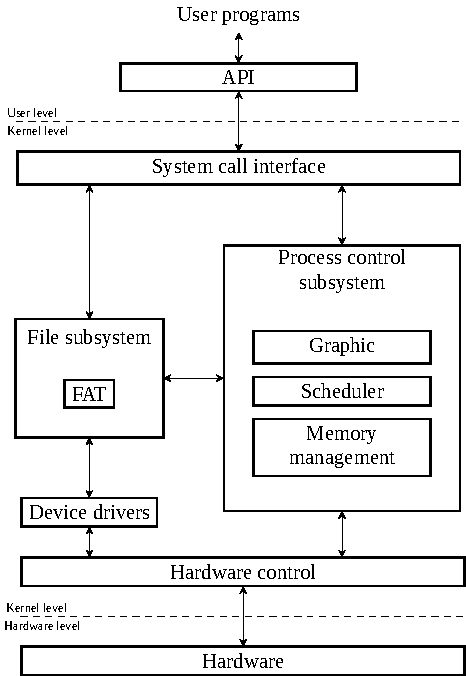
\includegraphics[scale=0.5]{../thesis/figs/kernel-block.pdf}
\caption{\emph{RongOS} overall design diagram.}
\end{figure}
\end{frame}


\section{Each Module Description in \emph{RongOS}}
\begin{frame}
\frametitle{Process Management}
Process management is the most complex part of operating system development, but this part
has far-reaching and extensive impact on the performance of the entire system.

Process management needs to complete the following work.
\begin{itemize}
\item Add task to task pool.
\item Scheduling running.
\item Sleeping task.
\item Process communication.
\end{itemize}


\end{frame}


\begin{frame}
\frametitle{Process Management}
\begin{figure}
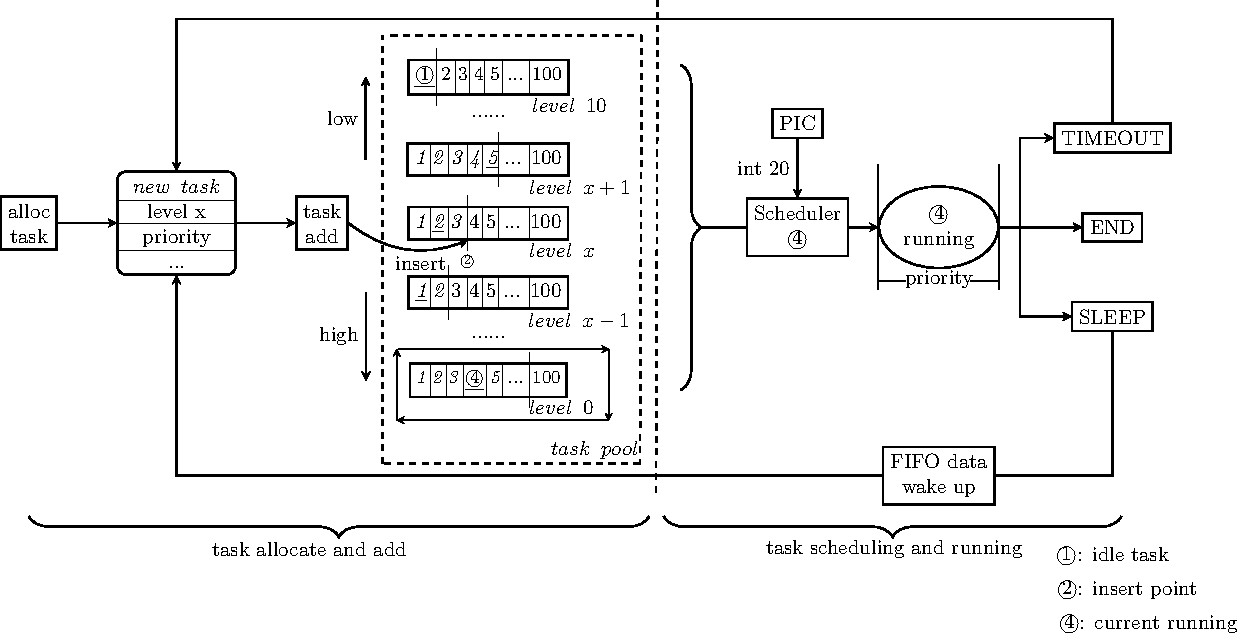
\includegraphics[scale=0.5]{../thesis/figs/process-manage.pdf}
\caption{Process management overall design diagram.}
\end{figure}
\end{frame}



\begin{frame}
\frametitle{Memory Management}
Memory management is the process of controlling and coordinating computer memory,
assigning portions called blocks to various running programs to optimize overall system
performance.

Memory management needs to complete the following work.

\begin{itemize}
\item Memory allocation.
\item Memory release.
\end{itemize}
The memory release is more complicated. It is divided into three situations.
\begin{itemize}
\item Can be merged with the previous one.
\item Can be merged with the latter
\item It can neither be merged with the latter one nor the former one.
\end{itemize}
\end{frame}

\begin{frame}
\frametitle{API}
The API is the interface that provides applications access to the operating system
kernel. More than twenty APIs are provided in \emph{RongOS}. Examples are as follows.

\begin{examples}
  \begin{itemize}
  \item void api\_putchar(int c): output a character c on the console window.
  \item void api\_putstr0(char *s): ouput a string s on the console window.
  \item int api\_getkey(int mode): accept keyboard input, mode indicates whether the
    keyboard is sleeping.
  \item ......
  \end{itemize}
\end{examples}

\end{frame}

\begin{frame}
  \frametitle{FAT}
  The FAT records which blocks the files are stored in. The file system of this system is
  relatively simple and only supports FAT.

  The main functions are as follows.
  \begin{itemize}
  \item file\_readfat: read FAT table.
  \item file\_loadfile: load file.
  \item file\_search: search file.
  \end{itemize}
  
  
\end{frame}

\begin{frame}
  \frametitle{Driver}
  In computing, a device driver is a computer program that operates or controls a
  particular type of device that is attached to a computer. A driver provides a software
  interface to hardware devices, enabling operating systems and other computer programs to
  access hardware functions without needing to know precise details of the hardware being
  used.

  There are several device drivers in \emph{RongOS}.
  \begin{itemize}
  \item Keyboard.
  \item Mouse.
  \item Palette.
  \end{itemize}
\end{frame}
\begin{frame}
  \frametitle{Graphic Management}
  Usually graphics management is not the concern of the operating system kernel for Linux, but not for Windows. However,
  as a simple system with windows, it is necessary to give some instructions for graphic
  management.

  The main services provided by graphic management are as follows.
  \begin{itemize}
  \item Refresh the window.
  \item Set the height of window.
  \end{itemize}
  
\end{frame}

\begin{frame}
  \frametitle{Set Height of Window}
  \begin{figure}
    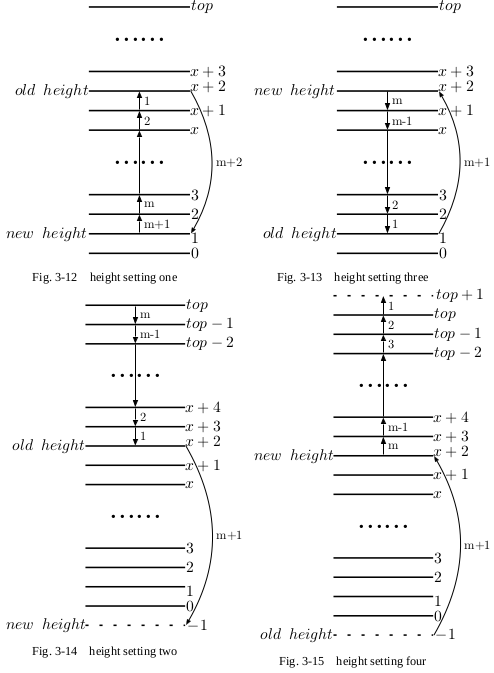
\includegraphics[scale=0.3]{four.png}
    \caption{Set the height of window.}
\end{figure}
  
  
\end{frame}


\section{APPs}

\begin{frame}
  \frametitle{Stars2}
  Obviously, application development is not the content of operating system development.
  But in order to verify that \emph{RongOS} is able to run programs developed in accordance with
  the \emph{RongOS} API, I decided to introduce an application implementation that is
  stars2. This application is to imitate the stars in the sky, I think the stars are a
  symbol of dreams, and I intend to end my thesis by showing dream. And developing an
  operating system is one of my dreams. The project ends but the dream will not.
\end{frame}

\begin{frame}
  \frametitle{Result of Stars2}
  \begin{figure}
    
\includegraphics[scale=2.4]{../thesis/figs/starts2.png}
    \caption{The running result of stars2.}
  \end{figure}
\end{frame}

\section{Postscript}

\begin{frame}
  \frametitle{Postscript — Why Rose}
  \begin{figure}
    
\includegraphics[scale=1.8]{whyRose.pdf}
  \end{figure}
  
\end{frame}

\begin{frame}
  \frametitle{Postscript — The Short Answer}
  \begin{figure}
    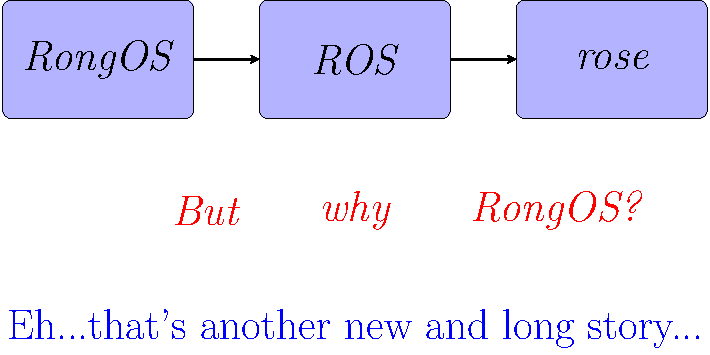
\includegraphics[scale=.9]{answer.pdf}
  \end{figure}
  
\end{frame}


\begin{frame}
  \frametitle{Postscript — Thanks}
  \begin{figure}
    
\includegraphics[scale=.8]{thanks.pdf}
  \end{figure}
  
\end{frame}


 
\end{document}


%%% Local Variables:
%%% mode: latex
%%% TeX-master: t
%%% End:
